\documentclass[12pt]{article}
\usepackage{amsmath,amsfonts,bbm,xfrac}
\usepackage{fancyhdr,enumitem,xcolor,subcaption}
\usepackage{graphicx} % Allows including images
\usepackage[left=3cm, right=3cm, top =2cm, bottom = 3cm]{geometry}
\usepackage{subfigure}
\usepackage[backend=biber,natbib, style=authoryear, maxcitenames = 4, maxbibnames = 10, uniquename=false, uniquelist=false]{biblatex}
\DeclareFieldFormat[misc,online,proceedings,report]{title}{\mkbibquote{#1}}
\DeclareFieldFormat*{citetitle}{\mkbibquote{#1\isdot}}
\addbibresource{bib.bib}

\newcommand{\E}{\mathbb{E}}


\pagestyle{plain}
%\setcounter{secnumdepth}{0}
\pagestyle{fancy} 
\rhead{Winter 2023} 
\chead{} 
\lhead{Econ 33550 - Spatial Economics} 
\lfoot{} 
\cfoot{\thepage} 
\rfoot{} 


\title{Spatial Economics - Problem Set I}
\author{Jose M. Quintero \and Jun Wong \and Rachel Williams}

\begin{document}

\maketitle

\section{Introduction}


Chicago is a widely studied city---it is unique in its spatial distribution of people and economic activity. Indeed, seminal work on city structure and segregation started from the examination of Chicago (CITE). The stark differences in economic activity and well-being across space in the city documented since XXX has persisted over time. Figure X shows the distribution of income across space in XXX and in 2010. Here, we build a quantitative spatial model to explain what fundamental forces drive these differences across space in Chicago in the cross-section.\footnote{Other than the fact that this assignment is a static exercise, we argue that dynamics do not add much to understanding the persistent spatial differences. If dynamics mattered more, we might expect the spatial distribution of activity to change.} We extend this model to include the agglomeration of two types of agents to study how including heterogeneous agents affects XXX. We are particularly interested in how different types of people sort across space in face of an amenity shock. We analyze the effects of the Obama Presidential Library construction in East Hyde Park, a relatively wealthier neighborhood in the south side of Chicago. We show that the implications of this is (DIFFERENT OR SAME) across the two models.

%% JW: So I think what would be really interesting is the discussion of what happens if we shocked a place with the lowest income with amenities vs shocking EHP?

% i usually hate these paragraphs. let me know how you feel.
In this introduction, we describe some diagnostics about the city of Chicago to motivate the model that we build in Section XX. Section YY describes the data and Section ZZ shows the results. Section BLAH concludes.

Some blah blah of what are we going to do, summarize the ingredients of the model, mention the data, limitations of the data if any, our counterfactual and main findings. This should be relatively fast. 

\section{Analysis of Chicago}

Chicago was incorporated as a city in 1837 for its unique location as an important trading post during the nation's westward expansion. Still today, 50 percent of all freight rail travels through Chicago. Chicago blossomed as a hub for trading agricultural products from the fertile soils of today's Midwest to markets on the east coast and in Europe. Successful rebuilding after the fire of 1871, Chicago earned the "Second City" mantra and entered into the global conversation by hosting the 1893 World's Fair in Jackson Park -- the very same park on which we will center on analysis. Steel, railroads, and especially meatpacking dominated Chicago's economy, but as the century changed Chicago became critical in fostering new industries such as the chemical industry, mail-order sales, telephone equipment and the radio. Chicago experienced a tectonic population shifts in the mid-20th century as millions of black Americans from the oppressed Jim Crow South moved north and settled in Chicago. Towards the end of the 1900s manufacturing industries left the crowded city in search of cheaper labor markets in the south and west. As documented by \citet{derenoncourt2022}, the local policy response in terms of shifting of public funds and redlining created a segregated city the remnants of which are still with us today: the north and northeast of the city are wealthier and has a disproportionate share of the White population; while the west and southwest of the city are poorer and has a disproportionate share of the Black population (Figure XX and XX). \citep{southside2022}
\begin{figure}[h!]
\centering
    \caption{Population by Race and Income}
    \begin{subfigure}[b]{0.52\textwidth}
         \centering
         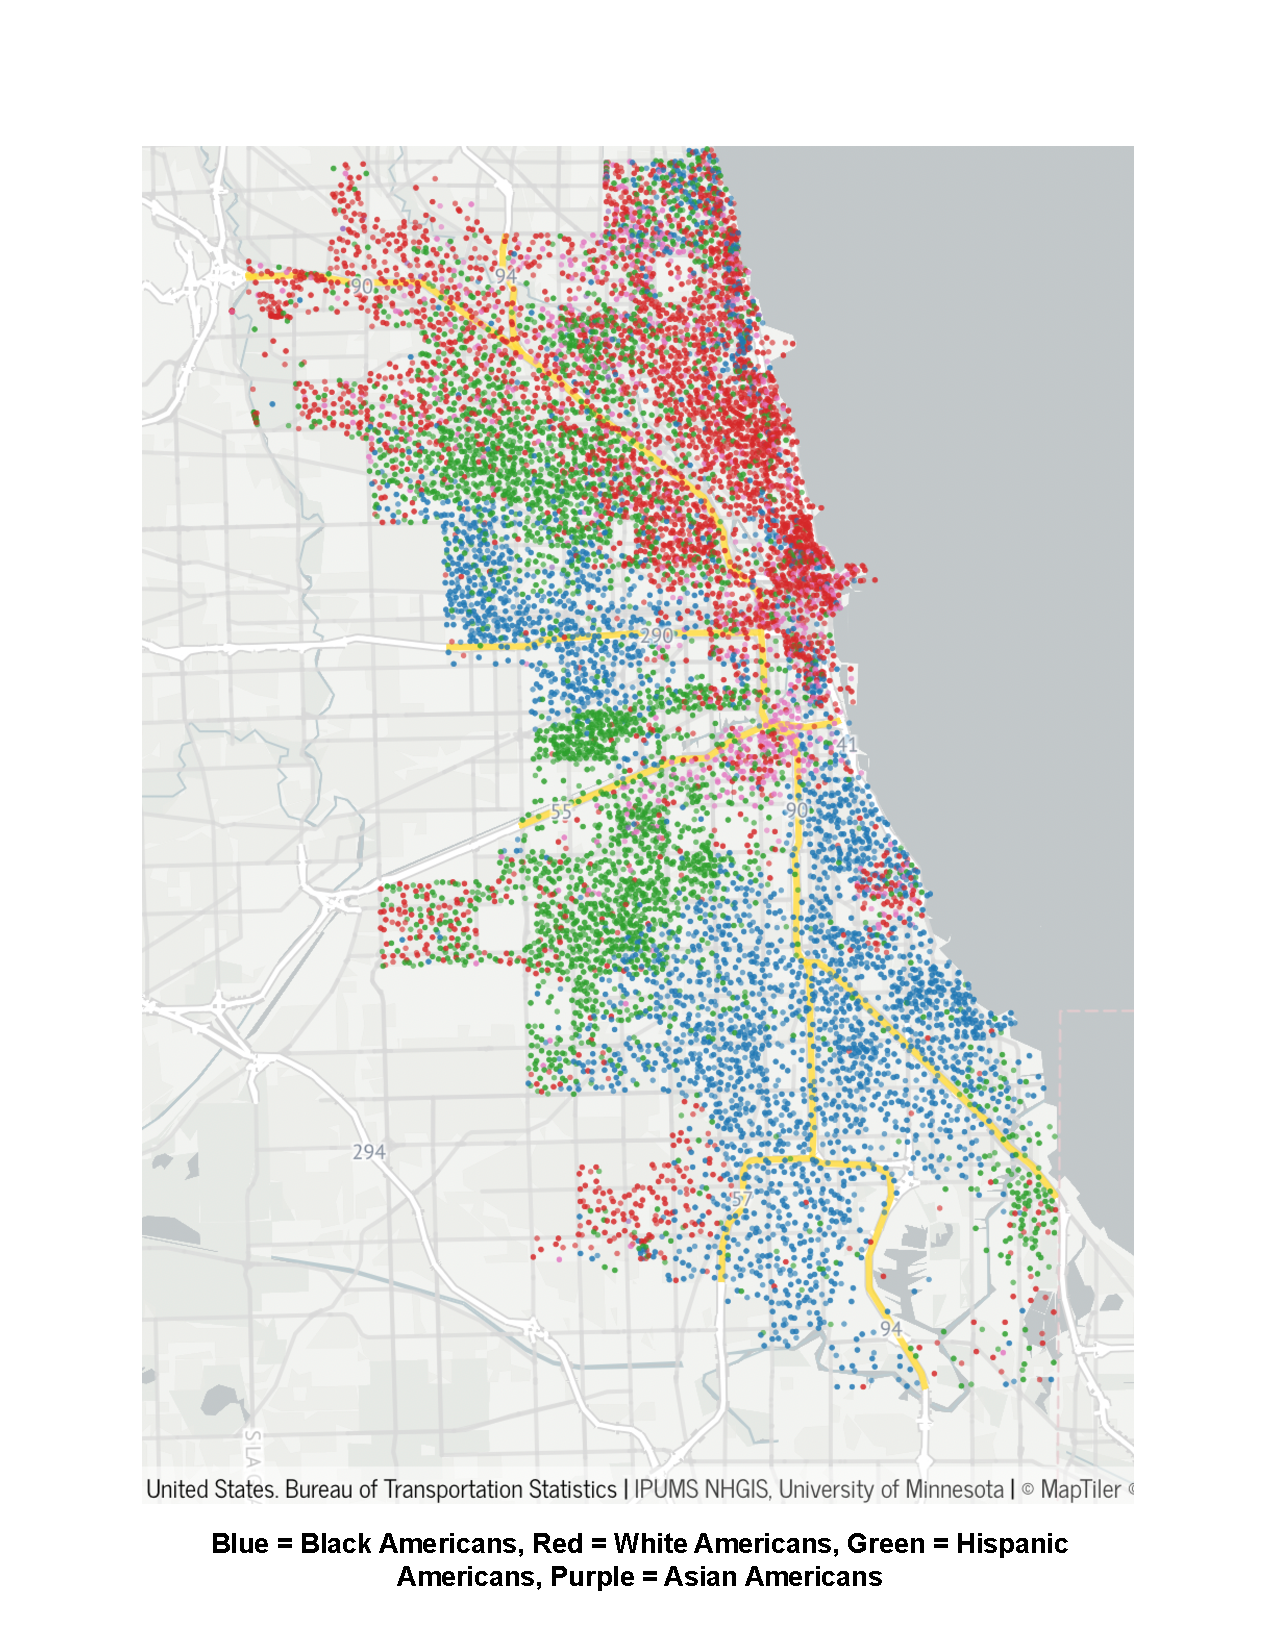
\includegraphics[width=\textwidth]{Pset1/Figures/racial_map.pdf}
         \label{fig:racial_divide}
    \end{subfigure}  
    \begin{subfigure}[b]{0.45\textwidth}
         \centering
         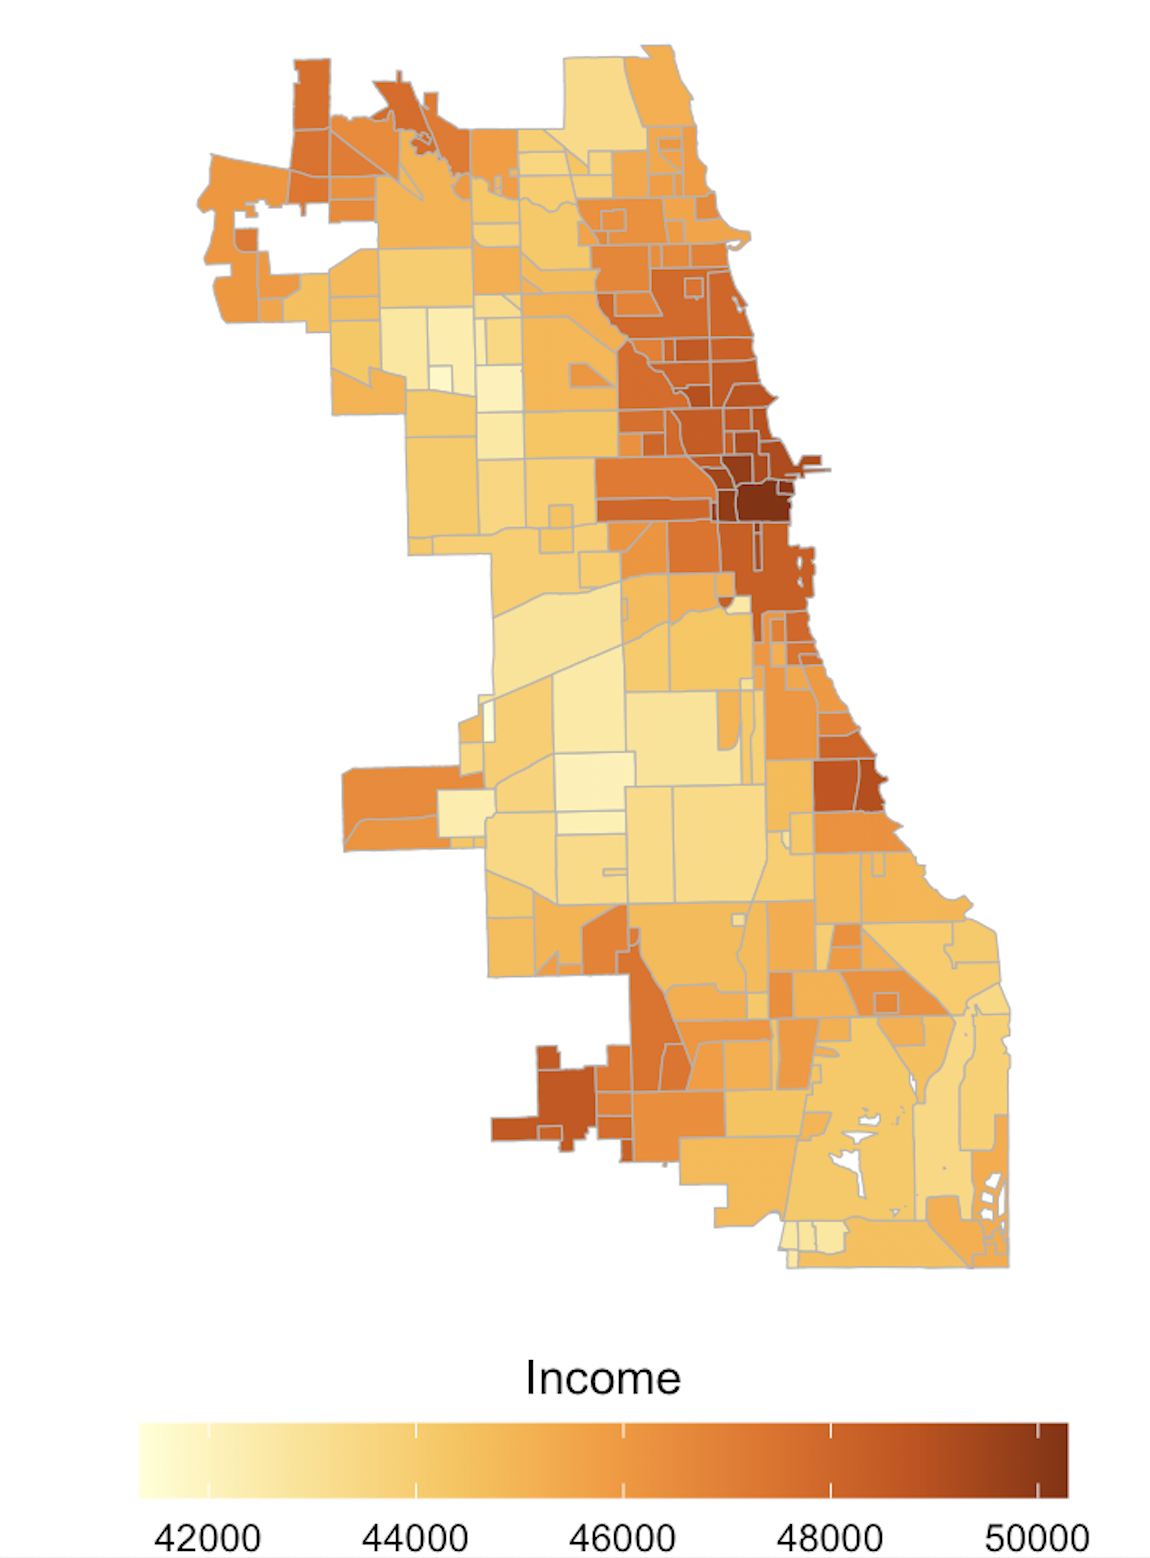
\includegraphics[width=\linewidth]{Pset1/Figures/income_map.png}
        \label{fig:income_divide}
    \end{subfigure}
\end{figure}



Housing prices similarly reflect this concentration of income in the northeast of Chicago (Figure XX). 

Employment is overwhelmingly concentrated in the downtown area, which offers the highest wages (Figure XX). Unsurprisingly, commuting probability from each neighborhood to downtown Chicago is correlated with average income (Figure XX). This is despite some neighborhoods having lower transport costs to the center of the city compared to others (Figure XX). 

Figure XX presents the commuting patterns of one of the poorest neighborhoods in the city, Englewood. While within Englewood, most of the commuters are going to downtown Chicago, we find that 24\% of these commuters work low-wage jobs. This stands in stark contrast to the commuting pattern of Lincoln Park---where the gravity remains in downtown Chicago. However, only 6\% of these commutes consist low-wage earners. Figure XX shows the share of commuters that have low-wage jobs by origin neighborhood. Unsurprisingly, low-wage earners reside primarily in the west and southwest of Chicago. 

Finally, we focus on the commuting characterisics of East Hyde Park. East Hyde Park is unique in that it is a high-income neighborhood located next to lower-income neighborhoods such as Woodlawn.\footnote{East Hyde Park is in the 95th percentile of the income distribution in Chicago.} Residents in East Hyde Park commute mostly to Hyde Park and downtown Chicago. It is not a neighborhood with a lot of employment opportunities: Consider its neighbor, Hyde Park, which attracts up to over 30\% of the commuters from certain neighborhoods. In contrast, East Hyde Park attracts at most 1\% the commuters from any given neighborhood. 
\section{The Model}


\subsection{Households}
A household is characterized by the neighborhood where she resides $i$ and where she works $j$. The household consume final good $c_{ij}$, land $H_{ij}$. Their utility is enhanced by neighborhood-specific amenities $B_i(R_i)$. Agents additionally have an idiosyncratic shock to their preferences $z_{ij}$ and $\kappa_{ij}\geq 1$ is the disutility of commuting from $i$ to $j$.  \\ 
\begin{equation}
    U_{ij}(z_{ij}) = \frac{B_iz_{ij}}{\kappa_{ij}}\left(\frac{c_{ij}}{\beta}\right)^{\beta}\left(\frac{H_{ij}}{1-\beta}\right)^{1-\beta}
\end{equation}
Following the trade literature, we assume that the shock is distributed Fréchet 
\begin{align*}
    \textcolor{blue}{F(s_{ij})} &\textcolor{blue}{= e^{\lambda_{ij}s_{ij}^{-\theta}}} & \textcolor{red}{F(s_{ij})} &\textcolor{red}{= e^{\lambda^o_{i}\lambda^d_js_{ij}^{-\theta}}}
\end{align*}
with $\theta>0$. 
The budget restriction for the agent is 
\begin{equation*}
    c + q_i^{r}H_{ij} = w_j
\end{equation*}
where I am normalizing the price of the consumption good and assume it is freely tradable within the city. Using profit maximization since the utility is a Cobb-Douglas, then the optimal decisions for $c$ and $H$ are  
\begin{align*}
    c_{ij} &= \beta w_j & H_{ij}&= \boxed{ \frac{(1-\beta)w_j}{q_i^{r}}}
\end{align*}
Then the utility for an agent living in neighborhood $i$, working in $j$ with a preference shock is 
\begin{equation}
    U_{ij}(z_{ij}) = \frac{B_iz_{ij}w_j}{\kappa_{ij}q_{i}^{1-\beta}}
\end{equation}
The intuition of the equation is pretty standard. Higher wages yield higher utility, higher commuting cost decreases utility, amenities increase utility, prices decrease utility and the preference shock increases utility. 

\subsection{Commuting Flows}
First, notice that the utility is also distributed Fréchet, 
\begin{align*}
    \Pr\left(U_{ij}\leq u\right) &= \Pr\left(\frac{B_iz_{ij}w_j}{\kappa_{ij}q_{i}^{1-\beta}}\leq u\right) 
    = \Pr\left( z_{ij}\leq \frac{u\kappa_{ij}q_i^{1-\beta}}{B_iw_j}\right) \\ 
    &= \exp\left(-\lambda_{ij}\left(\frac{B_iz_{ij}w_j}{\kappa_{ij}q_{i}^{1-\beta}}\right)^\theta u^{-\theta}\right) \\ 
    &= \exp\left(-\Phi_{ij}u^{-\theta}\right) = G_{ij}(u)
\end{align*}
Given this fact, the probability that an agent chooses to live in location $i$ and work in location $j$ is 
\begin{align*}
    \Pr\left(U_{ij}\geq \max_{r,s} U_{rs}\right) &= \Pr\left(U_{ij}\geq \max_{s} U_{is}\right)\Pr\left(U_{ij}\geq \max_{r} U_{kr},\quad\forall k\right) \\ 
    &= \prod_{s\neq i}\Pr\left( U_{ij}\geq U_{is}\right)\left[\prod_{r\neq j}\prod_{k}\Pr\left(U_{ij}\geq U_{kr}\right)\right] \\
    &= \int_0^{\infty}\theta\Phi_{ij}u^{-(\theta+1)}\prod_{s}\prod_{r}e^{-\Phi_{rs}u^{-\theta}} \mathrm{d}u \\ 
    &= \int_0^{\infty}\theta\Phi_{ij}u^{-(\theta+1)}e^{-\sum_{r}\sum_{s}\Phi_{rs}u^{-\theta}} \mathrm{d}u \\ 
    &= \frac{\Phi_{ij}}{\Phi}\int_0^{\infty}\theta\Phi u^{-(\theta+1)}e^{-\Phi u^{-\theta}} \mathrm{d}u \\ 
    &= \frac{\Phi_{ij}}{\Phi} = \pi_{ij}
\end{align*}
where $\Phi=\sum_{r}\sum_{s}\Phi_{rs}$. Using this result the probability an agent resides in location $i$ is 
\begin{equation*}
    \pi_{Ri} = \sum_{j=1}^N \pi_{ij} = \frac{1}{\Phi}\sum_{j=1}^N \Phi_{ij}
\end{equation*}
Similarly, the probability an agent works in location $j$ is
\begin{equation*}
    \pi_{Wj} = \sum_{i=1}^N \pi_{ij} = \frac{1}{\Phi}\sum_{i=1}^N \Phi_{ij}
\end{equation*}
Similar, conditional to living in location $i$, the probability of commuting to location $j$ is
\begin{align*}
    \pi_{ij\vert i} = \Pr\left(U_{ij}\geq \max_{r}U_{ir}\right) &= \Pr\left(\frac{B_iw_jz_{ij}}{d_{ij}q_i^{1-\beta}} \geq \max_{r} \frac{B_iw_rz_{ir}}{d_{ir}q_i^{1-\beta}} \right) \\ 
    &= \Pr\left(\frac{w_jz_{ij}}{d_{ij}} \geq \max_{r} \frac{w_rz_{ir}}{d_{ir}} \right) \\ 
    &= \int_0^\infty\Pr\left(\frac{w_jz_{ij}}{d_{ij}} \geq \max_{r} \frac{w_rz_{ir}}{d_{ir}}\bigg\vert z_{ij} \right) \mathrm{d}G_{ij}(z_{ij}) \\ 
    &= \int_0^\infty\prod_{r\neq j}\Pr\left(z_{ir}\leq \frac{w_jd_{ir}}{w_rd_{ij}}\bigg\vert z_{ij} \right) \mathrm{d}G_{ij}(z_{ij}) \\ 
    % &= \int_0^\infty \prod_{r=1}^N\exp\left(-\lambda_{ir}\left(\frac{w_jd_{ir}}{w_rd_{ij}}\right)^{-\theta}z_{ij}^{-\theta}\right)\lambda_{ij}\theta z_{ij}^{-(\theta+1)}\mathrm{d}z_{ij} \\ 
    &= \int_0^\infty \exp\left(-\left(\frac{w_j}{d_{ij}}\right)^{-\theta}z_{ij}^{-\theta}\sum_{r=1}^N\lambda_{ir}\left(\frac{d_{ir}}{w_r}\right)^{-\theta}z_{ij}^{-\theta}\right)\lambda_{ij}\theta z_{ij}^{-(\theta+1)}\mathrm{d}z_{ij} \\ 
    &= \frac{\lambda_{ij}\left(\sfrac{w_j}{d_{ij}}\right)^\theta}{\sum_{r=1}^N \lambda_{ir}\left(\sfrac{w_r}{d_{ir}}\right)^{\theta}}
\end{align*}
This expression allows to calculate the average wage of people residing in location $i$
\begin{equation*}
    \E\left[w_{Ri} \right] = \boxed{\sum_{j=1}^n w_j \pi_{ij\vert i}}
\end{equation*}

\subsection{Firms}

Firms produce a tradable good using a combination of labor $L_j$ and floor space $H_j^p$. To keep production simple, assume that the firms combine both inputs using a Cobb-Douglas production function with constant returns to scale
\begin{equation}
    Y_j = A_jL_j^\alpha \left(H_j^p\right)^{1-\alpha}, \quad\alpha\in(0,1)
\end{equation}
Let $y_t$ be the normalized output per unit of land, and $w_j$ the wage paid in location $j$. Then, the optimization problem for the firm is 
\begin{equation*}
    \max_{\ell_j} A_j\ell_j^\alpha - w_j\ell_j
\end{equation*}
The FOC implies the following wage
\begin{equation}
    w_j = \alpha A_j\ell_j^{\alpha-1}
\end{equation}
Assuming that $1-\alpha>\gamma$, the labor demand function for location $j$ is decreasing and has the form: 
\begin{equation*}
    L_j = \left(\frac{A_j\alpha}{w_j}\right)^{\frac{1}{1-\alpha}}H_j^p
\end{equation*}
Finally, as the firm has constant returns to scale, it will rent land until it hits zero profits. Then the demand for floor space it 
\begin{align*}
    q_j &= \frac{Y_j - w_jL_j}{H^p_j} \\ 
    &= (1-\alpha)A_j\ell_j^{\alpha} \\ 
    &= \boxed{(1-\alpha)A_j\left(\frac{\alpha A_j}{w_j}\right)^{\frac{\alpha}{1-\alpha}}}
\end{align*}

\subsection{Market Clearing Conditions}
For this section, we borrow the structure from the Berlin paper. Let $\theta_j$ be the share of floor space use for production. Then, for there not to be arbitrage, it has to be true that 
\begin{equation*}
    \theta_i = \begin{cases}
    1 &\mbox{if } q_i^p>q_i^r \\ 
    \in[0,1] &\mbox{if } q_i^p=q_i^r \\
    0 &\mbox{if } q_i^p<q_i^r 
    \end{cases}
\end{equation*}
Following the standard assumptions of urban models, floor space is supplied by competitive landlords. 

\subsection{Extension: Two types}
Now consider there are two types of agents that are imperfect substitutes to the firm. Specifically, the firm combines them with a Cobb-Douglas technology with 


\section{Counterfactual}

We examine the impact of the building Barack Obama’s Presidential Center in Jackson Park located in the East Hyde Park neighborhood. The project was announced in , it will be the first fully digitized presidential library. It will be built by the Lakeside Alliance and is on track to be completed by 2025. (CITE) An economic research firm commissioned by the University of Chicago found that of the economic impact of the library posit the library will attract approximately 800,000 annual visitors. This could translate into an annual economic impact of \$220 million and 1,900 net new jobs. In particular, South side neighborhoods should experience an estimated \$30 million more in spending by visitors to the Obama Library at local restaurants and retailers \citep{aeg2014}. This project will fundamentally change the landscape of the south side community. 

To put these numbers into perspective, \$30 million in spending would put east hyde park. The number of current commuters to East Hyde Park are XXX. How will positive amenity shock, drive up home prices and lead to gentrification on the south side?

\section{Data}

We combine ACS demographic data with Zillow home valuations in 2019. We get commuting data from XXX



\section{Quantification Strategy}



\section{Results}

\clearpage

\printbibliography


\end{document}
